\chapter{Introduction}


Today's Internet is an ``eyeball economy'' driven by applications, such 
as video streaming (e.g., the share of video traffic of all consumer Internet 
traffic  hit 70\% in 2015 and is forecasted to reach 82\% of consumer Internet traffic by 
2020~\cite{cisco-forecast-2015}) and Internet telephony (e.g., Skype users spend over 
2 billion minutes talking to each other every day~\cite{skype-2-billion-minutes}). 
As most applications rely on user engagement to generate revenues, 
it has become of paramount importance for the
application providers to ensure high user-perceived 
{\em Quality of Experience} ({\em QoE}) in order to maintain high user 
engagement~\cite{sigcomm13athula}.
For instance, recent research has shown that even one short video buffering 
interruption can lead to 39\% less time spent watching videos and 
cause substantial  revenue losses for ad-based video sites. 
Suboptimal QoE is similarly damaging for subscription-based 
service providers as well; e.g., our study with Microsoft Skype 
has shown that most Skype  users give low rating when experiencing over
1.2\% packet loss rate~\cite{via}.

Consequently, understanding and improving QoE of Internet applications 
has recently become a focus of academic and industry efforts. 
The trend is exemplified by the rapid growth in the number of recent
publications (e.g.,~\cite{sigcomm13athula,sigcomm12,
wang2014speedy,sigcomm11,eona,krishnan2013video}), workshops 
(e.g.,~\cite{workshop-wmust,workshop-fhmn,workshop-qoe}), 
as well as industry efforts (e.g.,~\cite{conviva,artizanetworks}) focusing on QoE optimization 
for a variety of applications such as video streaming, Internet telephony, mobile 
apps and web services.

%\begin{itemize}
%\item Overview of Internet applications: video streaming and internet telephony
%\item Re-architect the core -- high deployment cost
%\item Per-edge adaptation -- too narrow view
%\end{itemize}

%\section{Ensuring High QoE is Challenging}

\section{QoE Problems Today}

While there has been intense research towards improving Internet 
QoE over the past decades, existing approaches, however, have failed 
to deliver the QoE needed by today's applications. 
%Figure~\ref{fig:intro:badqoe} presents the QoE distribution and the 
%prevalence of bad QoE in video streaming and Internet telephony, 
%two of the most popular applications today.
%Figure~\ref{subfig:intro-badqoe-video-buffering} shows that among 
%over 300 million video sessions from 376 content 
%providers, 
For instance, our measurement study based on over 300 million 
video sessions from 376 content providers showed that
while most viewers did not experience noticeable re-buffering interruptions
(video stalls), 12\% video sessions spent over 1\% of time in re-buffering,
and 5\% sessions waste even 10\% of the view time in 
re-buffering~\cite{jiang2013shedding}, which could cause a significant 
fraction of viewers to quite watching the videos, especially for 
live content~\cite{sigcomm11}. 
%Similarly, Figure~\ref{subfig:intro-badqoe-skype-lossrate} shows that 
%among 430 million Skype calls that were not relayed by an intermediate
Similar pervasive QoE problems have been
shown in other applications as well. 
My study based on quality measurements from 430 million 
Skype calls showed that 17\% calls had experienced over 
1.2\% packet loss in the call's duration~\cite{via}, which 
according to user studies of VoIP\footnote{We use Internet telephony 
and VoIP interchangeably.} QoE~\cite{itu,cisco-voip} 
can cause very frustrating user experience.
Note that the packet loss rate is the average value over the
call's duration during which there may be transient spikes
(e.g., loss burst) resulting in even worse experience.


%\begin{figure}[t!]
%\captionsetup[subfigure]{justification=centering,farskip=-1pt,captionskip=5pt}
%\centering
%%\hspace{-0.5cm}
%\subfloat[Video streaming]
%{
%        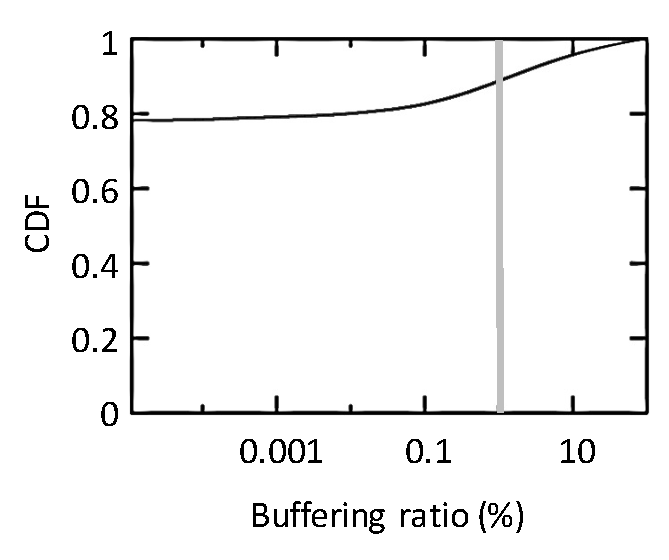
\includegraphics[width=0.35\textwidth]{figures/intro-badqoe-video-buffering.pdf}
%        \label{subfig:intro-badqoe-video-buffering}
%}
%%\hspace{-0.1cm}
%\subfloat[Internet telephony]
%{
%        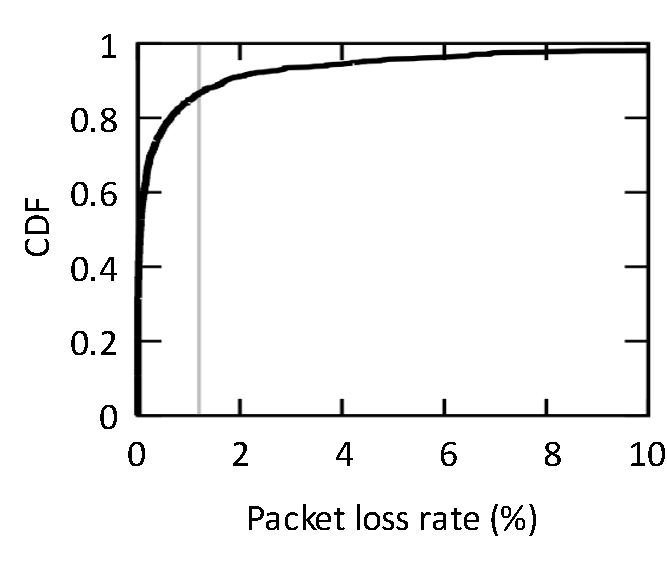
\includegraphics[width=0.35\textwidth]{figures/intro-badqoe-skype-lossrate.pdf}
%        \label{subfig:intro-badqoe-skype-lossrate}
%}
%%\vspace{-0.2cm}
%\caption{QoE distributions of video streaming and Internet telephony. 
%The figures shows that a substantial fraction of video sessions (12\%) 
%and VoIP calls (17\%) suffer from bad QoE (over 1\% buffering ratio 
%and 1.2\% packet loss rate, respectively).
%Buffering ratio is the fraction of video session duration spent in 
%re-buffering (video stalls), and is one of the key metrics of video 
%streaming QoE. 
%Packet loss rate is calculated over the call's duration, and is shown to 
%have significant impact on VoIP user experience.}
%%\vspace{-0.1cm}
%\label{fig:intro:badqoe}
%\end{figure}

To understand these QoE problems, we first shed light on
the fundamental limitations of prior approaches. 
These approaches can be broadly classified 
into two categories, with the key difference lying in their answers to
``{\em where to implement the functionality of QoE optimization}''.

%To see why prior research has failed to deliver desirable 
%QoE in a substantial fraction of cases, one has to understand
%their fundamental limitations. 
%Prior networking approaches to Internet QoE optimization can be 
%classified to two broad categories depending on the answer to the key 
%architectural 
%question ``{\em where to implement the functionality of QoE optimization?}''


\begin{itemize}
\item First, the {\em in-network approach} 
seeks to re-architect in-network devices such as routers, switches
and middleboxes, so that ISPs and middlebox services can provide
better or even guaranteed quality of service. 
Though this approach has inspired many influential projects 
(e.g.,~\cite{demers1989analysis,csfq,active-network}),
in-network devices have very {\em little visibility to user-perceived QoE}
as they have limited access to the client-side applications.
Moreover, it is hard, and increasingly so, to make significant changes 
or add new services to the network core in the real world. 

\item Second, the {\em endpoint approach} seeks to use
intelligent logic running in individual endpoints to cope with dynamic
network conditions and fully utilize the existing network resources.
This approach is pervasively used, ranging from
application-level protocols (e.g., video bitrate adaptation~\cite{dash}),
transport-level protocols (e.g., congestion control~\cite{jacobson1988congestion}),
down to link-level ones (e.g., wireless rate adaptation~\cite{holland2001rate}).
While having more direct insight to user-perceived QoE and arguably
more readily deployable than adding complexity to the network core, 
these endpoint-based schemes suffer from the key limitation 
that they can only use the 
{\em local information} observed by individual endpoints to
{\em react} to changes in network conditions or resource availability.
For instance, it takes a video player several seconds (or even tens of seconds)
to converge to an optimal combination of CDN and 
bitrate~\cite{dda-report}.
Moreover, we observe a growing decision space of potential control decisions 
to optimize application quality.
Consequently, trial-and-error strategies driven by single-session feedback are
fundamentally inefficient and slow in exploring the decision space and reacting to
changes. 
%Due to this limited knowledge of network conditions, it is difficult for 
%the endpoint adaptation to cope with the {\em growing decision space} 
%of potential control decisions to optimize application quality.

%of endpoint adaptation suffer from two limitations: 
%(1) it can only use the information visible to individual endpoint to react to dynamic network 
%conditions or resource availability,
%and (2) it typically uses manually designed strategies. 
%These two features inherently mismatch two recent trends of Internet applications
%First, we observe a {\em growing decision
%space} of potential control decisions to optimize application quality.
%Consequently, trial-and-error strategies driven by single-session feedback are
%fundamentally inefficient and slow in exploring the decision space and reacting to
%changes. For instance, it takes a video player several chunks (roughly 10s of
%seconds) to converge to an optimal combination of CDN and bitrate~\cite{dda-report}.
%Second,  we see an {\em increasing heterogeneity} in operating conditions, each requiring
%different control logic and parameters.  For instance, TCP parameters such
%as initial congestion window and AIMD parameters could be tweaked to work
%better in different operating conditions~\cite{remy,googleinitwindow}.
\end{itemize}

In essence, both in-network and endpoint approaches make trade-offs between
visibility of user-perceived QoE and visibility of 
network conditions, both of which, however, are necessary for achieving desirable QoE. 
In contrast, this dissertation approaches the placement of QoE optimization with a radically
different answer, and presents practical solutions to demonstrate that the new approach 
could get the best of both worlds.


\section{Data-Driven Paradigm in Networking}

This dissertation is inspired by a new paradigm called
{\em Data-Driven Networking} ({\em \ddn}), which
improves QoE by accurately predicting network conditions
based on {\em a real-time, global view of QoE measured from millions of 
end users~\cite{ddn-comsnet}.}
In essence, \ddn retains the ethos of the endpoint approach, 
while addressing its lack of
visibility to network condition by leveraging an expended view 
across many endpoints, thus achieving 
the best of both worlds of in-network and endpoint approaches.

\mypara{\ddn controller} 
The key component in \ddn is a logically centralized 
{\em controller}, which updates a real-time, 
global view of network conditions by 
QoE observed by applications running on 
many end users in real time, and uses this global view of
network conditions  to make  optimal decisions 
regarding configurations or adaptations of clients or application 
sessions\footnote{We use ``client'' to denote where a ``session'' 
is actually run.}.
A case in point is C3~\cite{c3}, where a video content provider 
collects session-level QoE measurements (e.g., buffering events) from 
the video players of its viewers, and predicts for any new session the best
bitrate and CDN selection based on the QoE measurements of 
history and concurrent video sessions.

\begin{figure}[t!]
\captionsetup[subfigure]{justification=centering,farskip=-1pt,captionskip=5pt}
\centering
%\hspace{-0.5cm}
\subfloat[Classic approaches.]
{
        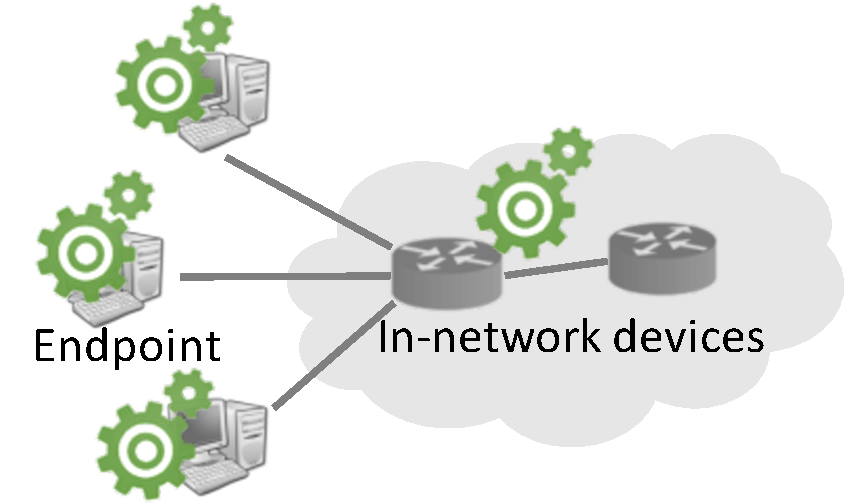
\includegraphics[width=0.4\textwidth]{figures/intro-classic.pdf}
        \label{subfig:problem-of-epsilon:change}
}
%\hspace{-0.1cm}
\subfloat[The new data-driven approach (\ddn).]
{
        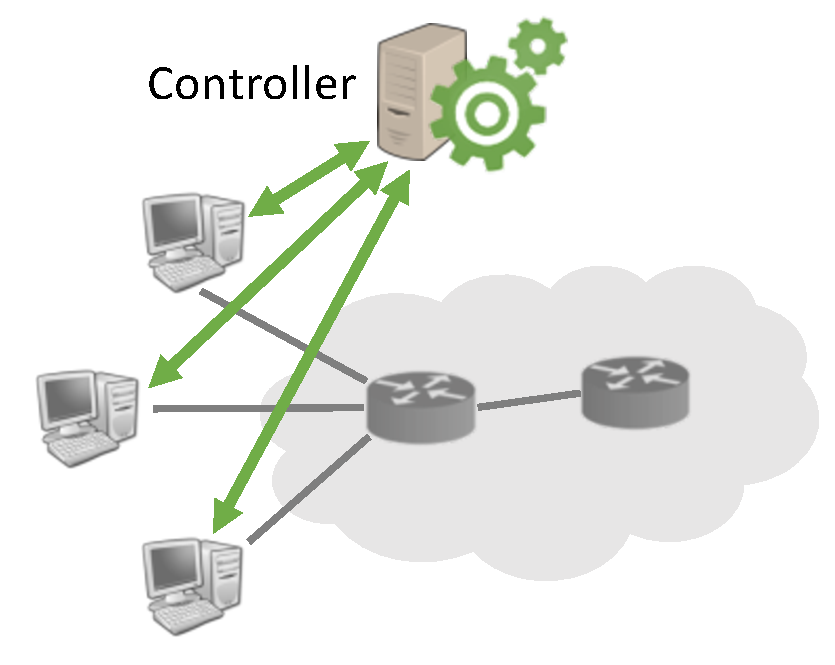
\includegraphics[width=0.4\textwidth]{figures/intro-ddn.pdf}
        \label{subfig:problem-of-slow:load}
}
%\vspace{-0.2cm}
\caption{Contrasting \ddn paradigm with classic approaches. 
The key different lies in where to implement the functionality of QoE optimization (symbolized by the gears): the classic approaches implement 
it in the network core or individual endpoints, whereas \ddn implements 
it in the controller that maintains a real-time global view of QoE of millions of endpoints.}
\vspace{-0.1cm}
\label{fig:intro:contrast}
\end{figure}

\mypara{Architectural advantages} 
Figure~\ref{fig:intro:contrast} crystallizes the contrast between
\ddn and classic approaches.
\ddn revisits the architectural question: ``where to implement the functionality of QoE 
optimization''.
While the classic approaches implement it in the network core or individual endpoints, 
\ddn implements the functionality of QoE optimization in the controller 
that maintains a real-time global view of QoE collected from
client-side applications running in millions of end users.
The design choice of moving the QoE optimization to the \ddn controller enjoys
two key architectural advantages.
\begin{itemize}
\item First, unlike the in-network approach, 
\ddn can measure user-perceived QoE directly as it has access to client-side applications,
and it is more readily deployable than 
re-architecting the network core.
\item Second, unlike the endpoint approach, 
\ddn compensates individual endpoints' lack of 
visibility of network conditions by a real-time, global view of QoE 
observed from many endpoints, thus addressing the key limitation of 
endpoint adaptation. 
%Instead of reacting to dynamic network conditions with 
%a local view, \ddn can {\em predict}  the QoE that a session would 
%experience if it uses certain decision.
\end{itemize}

\mypara{Technology trends} Compared to its precursor (e.g.,~\cite{spand,seshan1997spand}),
\ddn is fortuitously aligned with a confluence of recent  ``technology pulls''. 
First, many application providers today have widely deployed client-side 
instrumentations to collect massive real-time in-situ QoE data  (e.g.,~\cite{sigcomm11,via,imc12akamai,artizanetworks}). 
Second, the emergence of large-scale analytics systems provides the ability 
to extract insights efficiently from large corpses 
of data (e.g.,~\cite{spark}) and from streams of updates 
(e.g.,~\cite{zaharia2013discretized}). 
%Such ability enables optimal decision making based on
%real-time data-driven predictions~\cite{velox-cidr}.
Finally, control plane infrastructures have been built in many 
application and infrastructure providers, such as 
content providers~\cite{c3}, web services~\cite{footprint},
and CDNs~\cite{chen2015end,mukerjee2015practical}.

%\begin{itemize}
%\item {\em More measurement data in networking:}
%Many application providers today have widely deployed client-side 
%instrumentation to collect real-time performance data. 
%
%\item {\em ``Big data'' platforms finally a reality:}
%The emergence of large-scale analytics systems provides the ability to extract insights efficiently from large corpses 
%of data (e.g.,~\cite{spark}) and from stream of updates (e.g.,~\cite{dstream}). 
%Such ability enables optimal decision making based on real-time data-driven 
%predictions~\cite{velox}.
%
%\item {\em Wide use of control platforms:}
%Control plane platforms have been built by many individual subsystems (e.g., ISPs, video service providers and CDNs).
%
%\end{itemize}


%To take a concrete example, let’s think about Netflix player. 
%Traditionally, it takes a Netflix video player tens of seconds to converge to a good 
%quality, while in the new data-driven approach, Netflix can achieve much better 
%quality by using real-time quality measurement from many video players to directly 
%predict the best configuration for individual Netflix players.


%\subsection{Opportunities}

%\mypara{Opportunities of data-driven networking} 
%The data-driven approach is fortuitously aligned with several recent technology trends. Specifically, 
%
%\begin{itemize}
%\item {\em More measurement data in networking:}
%Many application providers today have widely deployed client-side 
%instrumentation to collect real-time performance data. \jc{examples}
%
%\item {\em ``Big data'' platforms finally a reality:}
%The emergence of large-scale analytics systems provides the ability to extract insights efficiently from large corpses 
%of data (e.g.,~\cite{spark}) and from stream of updates (e.g.,~\cite{dstream}). 
%Such ability enables optimal decision making based on real-time data-driven 
%predictions~\cite{velox}. \jc{examples}
%
%\item {\em Wide use of control platforms:}
%Control plane platforms have been built by many individual subsystems (e.g., ISPs, video service providers and CDNs). \jc{examples}
%
%\end{itemize}

\section{Contributions}

The main contribution of this dissertation lies in {\em the first suite of solutions to make \ddn 
practical}--we have demonstrated that QoE can be substantially improved by
leveraging QoE observed from millions of endpoints to maintain an up-to-date
global view of network conditions.
To achieve this, we identify its key technical challenges, address these 
challenges by novel algorithm and system designs that 
integrate machine-learning techniques with domain-specific  insights,
and use large-scale datasets and pilot 
deployments to demonstrate
the QoE improvement in the real world.

\mypara{Challenges}
While \ddn enjoys several advantages over 
classic approaches, we observe two fundamental challenges 
that are key to unleashing \ddn's full potential.
%We focus on two fundamental challenges unique to \ddn:

\begin{enumerate}

\item 
%{\em The need for expressive models} to capture complex factors affecting QoE. 
First, \ddn needs to extract actionable insights from the QoE measurement data, 
such as which sessions can be used to inform the decision of a new session.
%such as a predictive model to predict QoE based on session-level features, from 
%the data stream of QoE measurements. 
In short, we need {\em expressive models} to capture the potentially complex 
factors affecting QoE. 

\item 
%{\em The need for scalable platforms} to make real-time decisions with fresh data from geo-distributed clients.
Second, \ddn needs to turn the actionable insights into 
real-time control decisions to be performed by applications running in
geo-distributed clients. 
Therefore, we need {\em scalable platforms} that can respond to geo-distributed 
clients in real time with decisions based on fresh data from other clients.

\end{enumerate}

\mypara{Key insight}
In this dissertation, we address these challenges in practice by integrating 
several domain-specific insights in networked applications with 
standard machine learning algorithms and systems. 
%As a result, our 
%solutions achieve better QoE 
%than using off-the-shelf machine learning solutions. 
The unifying theme underlying these domain-specific insights is 
that there are {\em persistent structures} in the relationship
between session-level features, decisions, and QoE.
These structures help identify network sessions with similar 
QoE-determining factors, and that such structures tend to be 
persistent on timescales of tens of minutes.
To see an intuitive example of these persistent structures, let us consider 
a group of video sessions bottlenecked by a congested link.
The throughput of these flows may vary over time, but the fact
that these video sessions are bottlenecked by this congested link remains true 
for the whole duration of the congestion event.
In this example,  the persistent correlation between these sessions' 
network path and their QoE is a manifestation of the underlying congestion.
We will give a formal definition of persistent structures in
Section~\ref{sec:overview:unifying}.



%\begin{table}[]
%\centering
%\begin{tabular}{lll}
%\\ \hline
%{\bf Challenges} & {\bf Key ideas} & {\bf Published work}        \\ \hline\hline
%\begin{tabular}[c]{@{}l@{}}{\em Expressive models} for complex \\ QoE-determining factors\end{tabular}            & \begin{tabular}[c]{@{}l@{}}Use structures to identify sessions \\ with similar QoE-determining factors\end{tabular} & \begin{tabular}[c]{@{}l@{}}CFA~\cite{cfa}, VIA~\cite{via},  \\ CS2P~\cite{cs2p}\end{tabular}         \\ \hline
%\begin{tabular}[c]{@{}l@{}}{\em Scalable platforms} for real-time \\ decision making with fresh data\end{tabular} & \begin{tabular}[c]{@{}l@{}}Decouple offline structure learning \\ and the real-time decision making\end{tabular}    & \begin{tabular}[c]{@{}l@{}}Pytheas~\cite{pytheas}, CFA~\cite{cfa},  \\ C3~\cite{c3}, VDN~\cite{mukerjee2015practical}\end{tabular}\\ \hline
%\end{tabular}
%\caption{Summary of how the insight of persistent structures is used to address 
%the two key technical challenges of data-driven QoE optimization. The last 
%column shows the published work corresponding to these ideas.}
%\label{tab:contributions}
%\end{table}

\begin{figure}[t!]
\centering
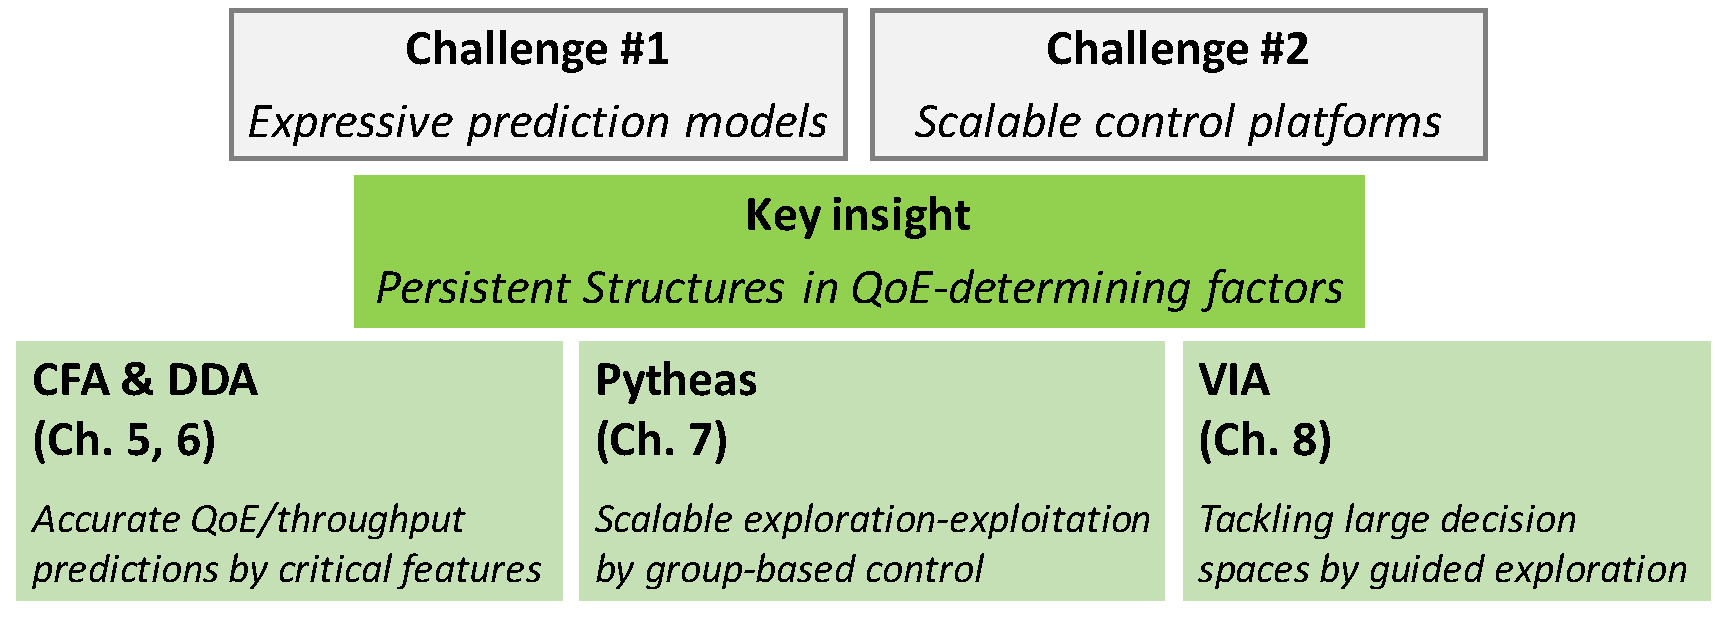
\includegraphics[width=0.7\textwidth]{figures/intro-contribution.pdf}
%\vspace{-0.3cm}
\caption{To address the key challenges
of \ddn, we have developed a suite of solutions by leveraging the domain-specific 
insight that QoE-determining factors
exhibit persistent structures.}
\label{fig:intro-contribution}
\end{figure}

\mypara{Proposed solutions}
%Table~\ref{tab:contributions} 
As illustrated in Figure~\ref{fig:intro-contribution}, 
the insight of persistent structures has inspired this dissertation's 
three major components 
to address the two aforementioned challenges in the context
of two popular Internet applications: Internet video and Internet telephony. 
At a high level, these domain-specific structures 
allow us to build expressive models that can identify network 
sessions with similar QoE-determining factors.
Moreover, because these structures are persistent, we can 
build scalable systems by decoupling the offline structure-learning 
process and the real-time decision making process.
%Based on these ideas, this dissertation has developed novel algorithms 
%and end-to-end systems, and deployed them in production settings to 
%improve QoE for Internet video streaming
%and Internet telephony. 
Next, we briefly describe the three major components that constitute 
this dissertation.



\begin{itemize}

\item {\bf Improving video QoE via expressive prediction models} 
(Chapter~\ref{ch:cfa} and~\ref{ch:dda}). 
Prior work has shown a substantial room for improving video QoE by 
dynamically selecting the optimal CDN and bitrate for individual video 
sessions based on a real-time global view of network 
conditions~\cite{sigcomm12}.
To realize this promise, we have developed CFA, a video QoE prediction 
system that can accurately predict the quality of a video client if it uses 
a certain CDN and bitrate; and DDA, a throughput prediction system
to accurately predict end-to-end throughput at the beginning of a 
 video session to help determine the highest-yet-sustainable initial bitrate.
In particular, CFA is inspired by the domain-specific insight of 
{\em persistent critical features}, an instantiation of persistent structures, that
each video session has a small set of critical features that ultimately 
determines its video quality, and these critical features change much 
more slowly than video quality, and thus can be practically 
learned from history data.
%This insight enables us to learn complex prediction models from long-term historical data (thus expressing complex relations between video quality and session features), and update the models by short-term historical data in near real time (thus capturing quality fluctuation as well).
%The insight of persistent critical features turns out to be more general than video streaming; e.g., I have also applied the same insight to accurate prediction of TCP throughput~\cite{cs2p}, which leads to 11\% higher video bitrate than state-of-the-art adaptive bitrate players (e.g., Netflix players) with no extra buffering.

\item {\bf Improving video QoE via exploration and exploitation at scale} 
(Chapter~\ref{ch:pytheas}). 
While CFA and DDA show promising QoE improvement by formulating the 
data-driven QoE optimization as a prediction problem, this formulation is necessarily 
incomplete, as it suffers from many known biases such as incomplete visibility, 
and cannot respond to sudden changes such as flash crowds.
Drawing a parallel from machine learning (e.g., ad recommendation), 
we argue that data-driven QoE optimization should instead be 
cast as a process of {\em real-time exploration and exploitation}. 
To apply this new abstraction to network applications at scale, 
we develop an end-to-end system, called Pytheas, based on 
another illustration of persistent structures that 
the sessions that exhibit similar QoE behavior will have similar network-level 
features (e.g., IP prefix), and thus their fresh data could be collected 
by the same geo-distributed front-end cluster close to the clients of
these sessions. Inspired by this insight, Pytheas uses a scheme called 
{\em group-based exploration and exploitation},  which decomposes the 
global exploration and exploitation process into 
subprocesses, each of which runs in a geo-distributed front-end cluster 
 and makes real-time decision for a group of similar sessions
based on their fresh measurement data.

\item {\bf Improving Internet telephony QoE in the face of large decision spaces} 
(Chapter~\ref{ch:via}).
The last project tackles a challenge of large decision spaces, which 
is particularly relevant in Internet telephony.
In the first large-scale study on VoIP quality, we found that 
%a substantial fraction of Skype calls suffer from poor network performance, 
%and that 
there is substantial room for improving Skype quality by routing each 
call through the optimal relay clusters in Microsoft's cloud.
However, identifying a close-to-optimal relay for each Skype call in practice 
is challenging, 
due to the sheer number of possible relay paths 
(in hundreds) and their dynamic performance (which could change 
on timescales of minutes). Neither prediction-based methods (e.g., 
CFA) nor those based on 
exploration and exploitation (e.g., Pytheas) would suffice to handle such a 
large decision space.
Our key insight to address this challenge is that, for each pair of caller 
AS and callee AS, there is a {\em small and stable subset} of relays that 
almost always contains the best relay path. These stable subsets of promising
relays are another manifestation of the persistent structures.
%This insight has two implications: 
%(1) because this subset of relays is stable, it can be learned from history; and 
%(2) because this subset has only a few relays (less than five), it can be explored efficiently even with limited data.
Inspired by these intuitions, we developed {VIA}~\cite{via}, 
a Skype relay selection system that achieves close-to-optimal quality 
using the concept of {\em guided exploration},
which learns a small set of promising relays for each 
AS pair based on long-term (e.g., daily) historical data, and 
explores these relays using most calls in real time.

\end{itemize}

%
%\jc{add why internet video, voip, and how to generalize}
Finally, while this dissertation has mostly focused on 
Internet video and Internet telephony, 
we observe similar data-driven opportunities in other applications
where solutions proposed in this dissertation can be readily 
deployable; e.g., CDN overlay routing~\cite{mukerjee2015practical}, 
web services~\cite{footprint}.
%some of which I have personally involved as well.
%We also observe parallel efforts that hint towards the potential
%of using a similar data-driven approach in other applications, such
%as web services~\cite{footprint}.
This suggests the potential {\em generalizability} of our solution to enable
data-driven QoE optimization in a broader set of challenges in 
networking and distributed systems.
%for particular applications might be 
%{\em generalized} to other applications and potentially to solutions for
%a broader set of challenges in networking and distributed systems.

\section{Evaluation}
%These improvements can lead to significant benefit for the application providers.

\mypara{Methodology}
%\mypara{Dataset}
To demonstrate the benefit of our solutions in realistic settings, 
our evaluation methodology combines real-world pilot deployment and 
emulation/simulation driven by large-scale datasets collected from real  users.
%this dissertation relies on either real-world pilot deployment or emulation 
%driven by large-scale datasets collected from real application traffic.
For instance, in Chapter~\ref{ch:cfa}, we integrated CFA in a production 
system~\cite{c3} that provided video optimization service for major content
providers in the US.
%to select CDNs and bitrates for real users for one of the biggest
%content providers in the US. 
We deployed CFA on one of these content providers to improve QoE for
150,000 sessions each day. We performed A/B tests (where each algorithm
was used on a random subset of clients) to evaluate
the improvement of CFA over baseline random decision
makers, which many video optimization services use
by default (modulo business arrangement like price).

\mypara{Metrics} 
In order to evaluate application QoE in a reliable 
and scalable fashion, this dissertation does not rely subjective QoE 
metrics (e.g., user-provided score), but focus on the metrics that can be
objectively measured and 
have been shown to have strong impact on user satisfaction 
and engagement.
For instance, video QoE is measured by buffering time, start-up delay,
and average bitrate, each of which has been shown to have strong
correlation with user engagement in multiple 
studies~\cite{sigcomm11,imc12akamai}.
While subjective metrics can directly reflect user satisfaction, we
choose to use these objectively measurable 
metrics as a proxy for real user satisfaction for two reasons:
(1) they can be passively collected on a large scale by instrumentation code 
running in client devices without any user input, and (2) they usually
are less noisy than subjective metrics which can be affected by factors
beyond the scope of this dissertation (e.g., content or personal preference).

%The QoE metrics against which different systems are compared 
%are objectively measurable metrics
%depend on the particular application under consideration.



%\mypara{Deployment}

\mypara{Summary of results}
%In order to evaluate the solutions proposed in this dissertation, 
%I focus on answering the following questions. 
In evaluating the solutions proposed in this dissertation, 
we focus on answering two questions.

\begin{itemize}

\item {\em How much can QoE be improved by the proposed solutions?}
The ultimate goal of \ddn is to improve QoE. 
Rather than evaluating multiple solution together, we examine the 
contribution of each solution by evaluating the incremental QoE 
improvement of adding one component at a time. 
For instance, by predicting the best CDN and bitrate selections based on 
a global view of network conditions, CFA reduces video re-buffering time 
on average by 32\% compared to a state-of-the-art client-side logic using 
local information (Chapter~\ref{ch:cfa});
and by re-casting the data-driven QoE optimization as a real-time 
exploration-and-exploitation process, Pytheas further reduces the 
re-buffering time on average by 30\% over CFA (Chapter~\ref{ch:pytheas}).
In Chapter~\ref{ch:via}, we show that VIA achieves better VoIP QoE
than CFA and Pytheas
by addressing the new challenge of large decision spaces in
Internet telephony.
Moreover, this dissertation also tries to identify the circumstances under which
the proposed solutions achieve more (or less) QoE improvement.
For instance, in Chapter~\ref{ch:via}, while 
we observe significant improvement of 
VIA on both international and domestic Skype calls, international calls
have a higher magnitude of improvement than domestic ones.

%Chapter~\ref{ch:cfa} shows that by predicting the best 
%CDN and bitrate selections based on a real-time, global view of network 
%conditions, CFA reduces re-buffering time on average by 32\% compared 
%with those selections made by a state-of-the-art client-side logic using 
%local information.
%Then Chapter~\ref{ch:pytheas} shows that Pytheas can further reduce the 
%re-buffering time on average by 30\% over CFA by recasting the 
%data-driven QoE optimization as a 
%real-time exploration-and-exploitation process.
%Finally, in Chapter~\ref{ch:via}, we show that VIA achieves better QoE
%than CFA and Pytheas in the context of a VoIP service 
%by reducing large decision spaces unique to Internet telephony.


\item {\em Can the proposed solutions be deployed at a real scale?}
Scalability is another critical metric to evaluate the proposed solutions. 
Any proposed algorithm must run at the scale of a large application 
provider.
%(e.g., YouTube has billions of video sessions per
%day over the world~\cite{youtube-stats}).
This means that the decisions must be made 
based on history data at a magnitude of hundreds GB or more, and 
these history data from geo-distributed 
clients must be up-to-date to maintain an accurate view of network conditions.
In Chapter~\ref{ch:cfa}, we show that CFA can update QoE 
prediction every tens of seconds with sub-second response 
time to geo-distributed clients, 
and in Chapter~\ref{ch:pytheas}, we show that Pytheas throughput 
scales horizontally with more machines in the controller, and that 
30 CloudLab instances can make decisions for the population of a site
like YouTube (5 billion sessions per day) with measurement data of 
concurrent sessions with less than a second of delay.

\end{itemize}



\section{Organization}
The rest of this dissertation is organized as follows.
Chapter~\ref{ch:related} begins with the background information of
Internet video and Internet telephony, including their QoE problems
today and current distribution infrastructures.
It then discusses two research directions closely 
relevant to this dissertation: 
quality optimization of Internet applications and applying data-driven 
techniques in networked systems.
In particular, it introduces a taxonomy of prior work on quality 
optimization, which emphasizes the trade-offs between 
more visibility of QoE feedback and more visibility of network
conditions.

Chapter~\ref{ch:overview} presents an overview of the main insight and 
ideas of this dissertation.
It begins with a formal description of the \ddn paradigm, some
concrete example applications that can benefit from \ddn, and a
perspective on its advantages over prior approaches.
It then elaborates the key technical challenges in making \ddn practical. 
Finally, it describes our key insight of persistent structures in 
QoE-determining factors, and how the insight inspires our ideas to 
address \ddn's challenges.
%It concludes with the contrast between the proposed solutions and classic 
%approaches, in order to elaborate their advantages and limitations.

Chapter~\ref{ch:measurement} presents a large-scale structural analysis
on the QoE problems of Internet video and Internet telephony in the wild.
It provides empirical evidence of the persistent structures in QoE-determining
factors. 

Chapters \ref{ch:cfa}, \ref{ch:dda}, \ref{ch:pytheas}, and \ref{ch:via} 
describe four important components of this dissertation: 
(1) CFA and DDA optimize video streaming quality by accurately predicting 
video QoE and end-to-end throughput using a global and real-time view of 
network conditions;
(2) Pytheas optimizes quality of Internet-scale applications by re-casting
the \ddn process as a real-time exploration-exploitation process 
over millions of geo-distributed clients at scale; and
(3) VIA optimizes network performance for Skype calls by selecting
the optimal relay clusters in the Microsoft cloud service.

Chapter~\ref{ch:concl} summarizes the contributions of the dissertation, 
discusses the limitations of the proposed solutions, and ends with future 
work.










